\documentclass[a4paper]{article}
\usepackage{tikz}
\usetikzlibrary{arrows.meta,
                positioning}

\begin{document}
    \begin{figure}[htb]
    \centering
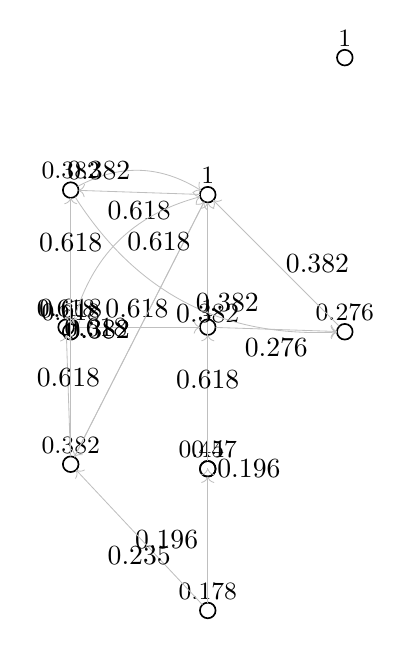
\begin{tikzpicture}[
node distance = 16mm and 16mm,
every edge/.style = {draw=gray!50, line width=0.3pt},
     N/.style = {circle, draw, semithick, inner sep=2pt, outer sep=0pt,
                 label={[font=\small, inner sep=1pt]above:#1}},
                        ]
\node (a1)   [N=1]  {};
\node (a2)   [N=0.276,below right=of a1] {};
\node (a3)   [N=0.447,below left=of a2] {};
\node (a4)   [N=0.178,below=of a3] {};
\node (a5)   [N=0.5,above=of a4] {};
\node (a6)   [N=1,above=of a5] {};
\node (a7)   [N=0.618,left=of a6] {};
\node (a8)   [N=0.382,below left=of a6] {};
\node (a9)   [N=0.382,above left=of a6] {};
\node (a10)  [N=0.618,below=of a9] {};
\node (a11)  [N=1,above right=of a1] {};
%
\path[->]
    (a1) edge node[left] {$0.382$} (a8)
    (a1) edge node[below] {$0.618$} (a9)
    (a2) edge node[right] {$0.382$} (a1)
    (a3) edge node[above] {$0.382$} (a1)
    (a4) edge node[left] {$0.196$} (a5)
    (a4) edge node[below] {$0.235$} (a8)
    (a5) edge node[above] {$0.618$} (a6)
    (a5) edge node[right] {$0.196$} (a3)
    (a6) edge node[below] {$0.276$} (a2)
    (a6) edge node[above] {$0.618$} (a7)
    (a7) edge node[left] {$0.618$} (a6)
    (a8) edge node[left] {$0.382$} (a1)
    (a8) edge node[above] {$0.618$} (a7)
    (a8) edge node[above] {$0.618$} (a9)
    (a9) edge node[above] {$0.618$} (a10)
    (a9) edge[bend left] node[left] {$0.382$} (a1)
    (a9) edge[bend right] node[right] {$0.382$} (a2)
    (a10) edge[bend left] node[right] {$0.618$} (a1)
    ;
\end{tikzpicture}
    \end{figure}
\end{document}